\chapter{Analytically Modified Integral Transform Expansion Technique}

\label{chapter_improved_expansions}

To achieve the expansion properties shown in Table
\ref{table_qualitative_comparison} for the AMITE technique
we develop expansions and approximations of the forms listed
in Chapter \ref{chapter_definitions}.  In all these expansions, we require
explicit formulas suitable for evaluation in arbitrary precision, yielding
expansions valid out to a tunable desired bound of validity $V$ which can be
made arbitrarily large.  The coefficients are allowed to depend on the order of
expansion $M$.
We present here an exposition of the general expansion
method which can be applied to a wide class of
activations.  We then begin application of the method
to our specific activations with an alternate
derivation of the Taylor series of $\tanh(v)$
formulated to illuminate the source of divergence in the
unmodified expansion, making apparent how it can be
modified to achieve our desired properties in Table
\ref{table_qualitative_comparison}.  We then apply the
method explicitly to $\relu(v)$, $\sech(v)$, $\tanh(v)$, $\sech^2(v)$,
and finally to a single hidden layer MLP as a whole.

\section{General Expansion Technique}
\label{section_method_technique}
Our general method for obtaining the coefficients
is as follows.  First, the function $\varphi$ to be
approximated is expressed via an integral transform of the form:
\begin{equation}
	\varphi(v) = \int_\mathbb{R} \! \Phi(\xi) f(\xi v) \mathrm{d}\xi.
\end{equation}
We find the Fourier transform family well suited to this step.
The kernel $f(\xi v)$ is then expanded via the truncated Taylor series
\begin{align}
	f(\xi v) &= \sum_{m=0}^M \tilde{f}(m) (\xi v)^m
	+ \Upsilon_M^{\{f\}}(\xi v),
	\label{eq_taylor_f} \\
	\varphi(v) &\simeq \int_\mathbb{R} \!
	\Phi(\xi) \sum_{m=0}^M \tilde{f}(m) (\xi v)^m \mathrm{d}\xi.
	\label{eq_phi_v_integral}
\end{align}
The remainder $\Upsilon_M^{\{f\}}(\xi v)$ is factored into parts
$P_M(\xi v)$ and $Q_M(\xi v)$
that increase with and without bound respectively
\begin{equation}
	\label{eq_remainder_factorization}
	\Upsilon_M^{\{f\}}(\xi v) = P_M(\xi v) Q_M(\xi v) .
\end{equation}

The dominating term $Q_M(\xi v)$ is set equal to a constant $C$ and
solved for $\xi$ to determine a suitable limit $\xi = \rho(M)$ of
integration for (\ref{eq_phi_v_integral}) which remains in the
region of convergence of (\ref{eq_taylor_f}), i.e., $\xi = Q_M^{-1}(C) / v$.
In cases where $v$ can take on one of many values, the limit of
integration can be defined with respect to its maximum value $V$
to err on the side of safety.
\begin{equation}
	\rho_V(M) = Q_M^{-1}(C)/V
\end{equation}
The integral of (\ref{eq_phi_v_integral}) can then be rewritten as
\begin{equation}
	\varphi(v) \simeq
	\sum_{m=0}^M \tilde{f}(m) v^m
	\int_{-\rho_V(M)}^{\rho_V(M)} \!
	\Phi(\xi)\xi^m \mathrm{d}\xi. \label{eq_phi_v_intermediate_expansion}
\end{equation}
where the exchange of the summation and the integral is permitted since
the integral is bounded to the convergent region $(-\rho_V(M), \rho_V(M))$.
Solving the remaining integral yields an approximation in the desired form of
(\ref{eq_alpha_expansion}).

By noting the parts of (\ref{eq_phi_v_integral}) left out by the
adjustments an exact expression for the
remainder $H_M^{\{\varphi\}}(v)$ is revealed
\begin{equation}
	H_M^{\{\varphi\}}(v) = \
	\int_{-\rho_V(M)}^{\rho_V(M)} \!
	\Phi(\xi)\Upsilon_M^{\{f\}}(\xi v) \mathrm{d}\xi \\
	+ 
	\int_{-\infty}^{-\rho_V(M)} \!
	\Phi(\xi)f(\xi v) \mathrm{d}\xi
	+ 
	\int_{\rho_V(M)}^{\infty} \!
	\Phi(\xi)f(\xi v) \mathrm{d}\xi \label{eq_general_remainder}
\end{equation}
such that the expansion and its coefficients are given as
\begin{align}
	\begin{split}
		\label{eq_alpha_expansion_full}
		\varphi(v) &= \sum_{m=0}^{M} \alpha_m(M) v^m + H_M^{\{\varphi\}}(v) \\
		&\simeq \sum_{m=0}^{M} \alpha_m(M) v^m \ \ \forall \ \ |v| < V
	\end{split}
	\\
	\begin{split}
		\alpha_m(M) &= \tilde{f}(m)
		\int_{-\rho_V(M)}^{\rho_V(M)} \!
		\Phi(\xi)\xi^m \mathrm{d}\xi \label{eq_alpha_coef_general_form}
	\end{split}
\end{align}

\section{Alternate Taylor Series Derivations}
To show how the AMITE expansion technique relates to the Taylor series, it is instructive
to derive the Taylor series of some of our target functions in a manner which makes apparent
where they can be modified to achieve the desired properties.  Instead
of employing the usual Taylor series formula, we express the target functions in terms of
their known Fourier transforms and then derive their Taylor series from the Taylor series of
the transform kernels.

\subsection{Hyperbolic Secant}
We derive the Taylor series of $\sech(v)$ by expressing
it in terms of its Fourier transform. Identities from
\cite{bateman_integral} yield
\begin{align}
    \sech(v) &= \lim_{\rho \to \infty}
    \int_0^\rho \!
    \sech\left(\frac{\pi}{2}\xi\right)\cos(\xi v) \,
    \mathrm{d}\xi.
\end{align}
Expanding the kernel $\cos(\xi v)$ to a partial sum yields
\begin{align}
	\sech(v) &\simeq
	\lim_{\rho \to \infty}
	\sum_{m=0}^{M}
	\frac{(-1)^m v^{2 m}}{(2 m)!}
	\int_0^\rho \!
	\xi^{2 m}\sech\left(\frac{\pi}{2}\xi\right)
	\mathrm{d}\xi. \label{eq_sech_intermediate_taylor}
\end{align}
Noting the identity
\begin{align}
\int_0^\infty \!
\xi^{2 m} \sech\left(a \xi\right)
\mathrm{d}\xi =
\left(\frac{\pi}{2a}\right)^{2m + 1}
\left|E_{2m}\right|,
\end{align}
from \cite{gradshtein_table_2007} yields the familiar Taylor series
\begin{align}
	\sech(v) \simeq
	\sum_{m=0}^{M}\frac{E_{2 m} v^{2 m}}{(2 m)!},
	\quad \forall \quad |v| < \frac{\pi}{2}.
\end{align}

\subsection{Hyperbolic Tangent}
We derive the Taylor series of $\tanh(v)$ by expressing
it in terms of its Fourier transform. Identities from
\cite{bateman_integral} yield
\begin{align}
	\tanh(v) &= \lim_{\rho \to \infty}
	\int_0^\rho \!
	\csch\left(\frac{\pi}{2}\xi\right)\sin(\xi v) \,
	\mathrm{d}\xi.
\end{align}
Expanding the kernel $\sin(\xi v)$ to a partial sum yields
\begin{equation}
	\tanh(v) \simeq \\
	\lim_{\rho \to \infty}
	\sum_{m=1}^{M}
	\frac{(-1)^{m-1} v^{2 m - 1}}{(2 m - 1)!}
	\int_0^\rho \!
	\xi^{2 m - 1}\csch\left(\frac{\pi}{2}\xi\right)
	\mathrm{d}\xi.  \label{eq_tanh_intermediate_taylor}
\end{equation}
Noting the identity
\begin{equation}
	\begin{split}
		\int_0^{\infty} \! \xi^{2 m - 1} \csch(a \xi) \mathrm{d}\xi = 
		\frac{2^{2 m} - 1}{2 m}
		\left(\frac{\pi}{a}\right)^{2m}
		|B_{2m}|,
	\end{split}
\end{equation}
from \cite{gradshtein_table_2007} and applying to (\ref{eq_tanh_intermediate_taylor})
yields the familiar Taylor series
\begin{equation}
	\begin{split}
		\tanh(v) \simeq
		\sum_{m=1}^{M}\frac{2^{2m}(2^{2m}-1)B_{2m}v^{2m-1}}{(2m)!},
		\quad \forall \quad |v| < \frac{\pi}{2}.
	\end{split}
\end{equation}

\subsection{Hyperbolic Secant Squared}
We proceed similarly for the hyperbolic secant squared.
\begin{align}
	\sech^2(v) &= \lim_{\rho \to \infty}
	\int_0^\rho \!
	\xi\csch\left(\frac{\pi}{2}\xi\right)\cos(\xi v) \,
	\mathrm{d}\xi, \\
	\sech^2(v) &\simeq
	\lim_{\rho \to \infty}
	\sum_{m=0}^M
	\frac{(-1)^m v^{2 m}}{(2 m)!}
	\int_0^\rho \!
	\xi^{2 m + 1}\csch\left(\frac{\pi}{2}\xi\right)
	\mathrm{d}\xi \label{eq_sech2_intermediate_taylor} \\
	\sech^2(v) &\simeq
	\sum_{m=0}^{M} \frac{2^{2m+1}(4^{m+1}-1)B_{2m+2}v^{2m}}{(m+1)(2m)!},
	\quad \forall \quad |v| < \frac{\pi}{2}.
\end{align}

Noting that the manipulations of Eqs. (\ref{eq_sech_intermediate_taylor}, \ref{eq_tanh_intermediate_taylor}, \ref{eq_sech2_intermediate_taylor})
are only valid within the convergent regions of the Taylor
expansions of the kernels, $\cos(\xi v)$ and $\sin(\xi v)$, illuminates the source of
the divergence for $|v|\geq \pi/2$. We illustrate in the following section
how this can be mitigated while preserving accuracy over
an arbitrary interval.


\section{Modifying the Limits of Integration}
To modify the integrals of Eqs. (\ref{eq_sech_intermediate_taylor}, \ref{eq_tanh_intermediate_taylor}, \ref{eq_sech2_intermediate_taylor})
so that the resulting expansions are valid for $|v| \geq \frac{\pi}{2}$ we require
a suitable upper bound $\rho$ accounting for the domain of validity
of the $M$-term partial sum expansions of the kernels. Following Section
\ref{section_method_technique} we begin by factoring the remainders of
the partial sums to consider the dominant factors which contribute to
their divergence. We treat both  $\sin(\xi v)$ and $\cos(\xi v)$ which
we will employ in the next sections to expand $\sech(v)$, $\tanh(v)$, $\sech^2(v)$ and $\relu(v)$.
We begin with the partial sum formulas
\begin{align}
	\cos(u) &= 
	\sum_{m=0}^{M}\frac{(-1)^m u^{2 m}}{(2 m)!}
	+ \Upsilon_M^{\{\cos\}}(u), \label{eq_partial_sum_cos} \\
	\sin(u) &= 
	\sum_{m=0}^{M}\frac{(-1)^m u^{2 m + 1}}{(2 m + 1)!}
	+ \Upsilon_M^{\{\sin\}}(u), \label{eq_partial_sum_sin}
\end{align}
having remainders given by
\begin{align}
	\begin{split}
		\Upsilon_M^{\{\cos\}}(u) = 
		(-1)^{M+1} u^{2M+2}
		\sum_{m=0}^{\infty}
		\frac{(-1)^m u^{2m}}{(2m+2M+2)!}, \\
	\end{split}
	\\
	\begin{split}
		\Upsilon_M^{\{\sin\}}(u) = 
		(-1)^{M+1} u^{2M+3}
		\sum_{m=0}^{\infty}
		\frac{(-1)^m u^{2 m}}{(2m+2M+3)!}.
	\end{split}
\end{align}
Factoring the remainders in the form of
(\ref{eq_remainder_factorization}) yields
\begin{align}
	\begin{split}
		\Upsilon_M^{\{\cos\}}(u) = 
		\frac{(-1)^{M+1} u^{2M+2}}{(2M + 2)!}
		\ {}_{1}F_{2}
		\left(1; M+2, M+\frac{3}{2}; -\frac{u^2}{4}\right), 
		\label{eq_cos_remainder_hypergemom}
	\end{split}
	\\
	\begin{split}
		\Upsilon_M^{\{\sin\}}(u) = 
		\frac{(-1)^{M+1} u^{2M+3}}{(2M+3)!}
		\ {}_{1}F_{2}
		\left(1; M+2, M+\frac{5}{2}; -\frac{u^2}{4}\right)
		\label{eq_sin_remainder_hypergeom}.
	\end{split}
\end{align}

As $u$ tends to infinity the hypergeometric factors in
(\ref{eq_cos_remainder_hypergemom}) and (\ref{eq_sin_remainder_hypergeom})
tend to zero and the outer factors
\begin{equation}
	Q_M^{\{\cos\}}(u) = \frac{u^{2M+2}}{(2M+2)!}, 
	\quad Q_M^{\{\sin\}}(u) = \frac{u^{2M+3}}{(2M+3)!},
\end{equation}
tend to infinity. Noting that the outer factors drive the remainders'
growth we define the range of validity of the partial sums
in (\ref{eq_partial_sum_cos}) and (\ref{eq_partial_sum_sin})
to be all $u$ such that
$Q_M^{\{\cos\}}(u) < 1$ and $Q_M^{\{\sin\}}(u) < 1$
respectively.  This yields the required bounds on the
domain of validity of each partial sum:
\begin{align}
	\cos(u) &\simeq \sum_{m=0}^M \frac{(-1)^m u^{2m}}{(2m)!}
	\quad \forall \quad u < ((2M+2)!)^{\frac{1}{2M+2}}, \\
	\sin(u) &\simeq \sum_{m=0}^M \frac{(-1)^m u^{2m+1}}{(2m+1)!}  
	\quad \forall \quad u < ((2M+3)!)^{\frac{1}{2M+3}}.
\end{align}

Noting the argument to the kernel in Eqs. (\ref{eq_sech_intermediate_taylor}, \ref{eq_tanh_intermediate_taylor}, \ref{eq_sech2_intermediate_taylor})
is $u = \xi v$, and adjusting for the maximum value $V = \max(v)$, we
let $\sigma$ and $\tau$ denote the required upper bounds for
integrals in the forms $\int \Phi(\xi)\cos(\xi v)\mathrm{d}\xi$ and
$\int \Phi(\xi)\sin(\xi v)\mathrm{d}\xi$
respectively:
\begin{align}
	\sigma = \frac{((2M+2)!)^{\frac{1}{2M+2}}}{V}, \ \ 
	\tau = \frac{((2M+3)!)^{\frac{1}{2M+3}}}{V}.
	\label{eq_range_of_validity}
\end{align}

\section{An Improved Hyperbolic Secant Expansion}
Having identified the appropriate bound, $\sigma$, for integrals having
kernels $\cos(\xi v)$ we can now return to
(\ref{eq_sech_intermediate_taylor}) and integrate the component
$
\int \!
\xi^j\sech\left(\frac{\pi}{2}\xi\right)
\mathrm{d}\xi
$
from $0$ to $\sigma$ to yield the desired formulas for the
coefficients $S_{2m}(M)$.
\begin{gather}
	\begin{split}
		\label{eq_sech_expansion_full}
		\sech(v) &= \sum_{m=0}^{M} S_{2m}(M) v^{2m} + H_M^{\{\sech\}}(v) \\
		&\simeq \sum_{m=0}^{M} S_{2m}(M) v^{2m} \quad \forall \quad |v| < V,
	\end{split}
	\\[1ex]
	\begin{split}
		S_{2m}(M) = \frac{E_{2m}}{(2m)!}
		+ \frac{(-1)^{m+1}4}{\pi} \sum_{k=0}^{2m}
		\frac{2^k \sigma^{2m-k}
			\mathrm{Ti}_{k+1}\left(e^{-\frac{\pi \sigma}{2}}\right)}
		{\pi^{k}(2m-k)!}.
		\label{eq_xi_sech_solution3}
	\end{split}
\end{gather}
Here, $\mathrm{Ti}_s(z) = \frac{1}{2i}(\polylog_s(iz) - \polylog_s(-iz))$ denotes the
Inverse Tangent Integral. We note that this expression represents a precisely defined adjustment on
the Taylor series of $\sech(v)$.  The result of (\ref{eq_xi_sech_solution3}) is
derived fully in Appendix \ref{appendix_expansions_detail}. The precise
remainder then follows directly from application of
(\ref{eq_general_remainder}):
\begin{align}
	\begin{split}
		&H_M^{\{\sech\}}(v) = \int_\sigma^{\infty} \!
		\sech\left(\frac{\pi}{2}\xi\right)
		\cos(\xi v) \mathrm{d}\xi
		\label{eq_sech_remainder2}
	\end{split}
	\\
	\begin{split}
		& \quad\quad + \frac{(-1)^{M+1}v^{2M+2}}{(2M+2)!} \int_0^{\sigma} \!
		\xi^{2M+2} \sech\left(\frac{\pi}{2}\xi\right)
		{}_{1}F_{2}\left(1; M+2, M+\frac{3}{2}; -\frac{v^2 \xi^2}{4}\right) \mathrm{d}\xi. \label{eq_sech_remainder1}
	\end{split}
\end{align}

The second term (\ref{eq_sech_remainder1}) dominates for
large $v$ due to the $v^{2M+2}$ factor, causing the expected divergence
for $|v| \geq V$.  Since (\ref{eq_sech_remainder1}) follows directly
from the Taylor remainder $\Upsilon_M^{\{\cos\}}(\xi v)$ it is by
definition small for $v$ within the region of convergence.
Meanwhile, the first term (\ref{eq_sech_remainder2})
dominates for small $v$ leading to Gibbs-like oscillation of the
error for $|v| < V$.  Noting this effect, the integral of
(\ref{eq_sech_remainder2}) can be solved exactly to analyze the
error inside the region of convergence for an $M$ term expansion.
Let $I_M^{\{\sech\}}(v)$ denote this error component:
\begin{gather}
	\begin{split}
		\label{eq_lerch_error_part_sech}
		&I_M^{\{\sech\}}(v) = \int_\sigma^{\infty} \!
		\sech\left(\frac{\pi}{2}\xi\right)
		\cos(\xi v) \mathrm{d}\xi \\
		&= 2 \sech(v)
		 - \frac{1}{\pi}\left(
		    \left( e^{\pi\sigma}\right)^{\frac{1}{2} + \frac{iv}{\pi}}
		    \Phi\left(-e^{\pi \sigma}, 1, \frac{1}{2} + \frac{iv}{\pi}\right)
		    +
		    \left( e^{\pi\sigma}\right)^{\frac{1}{2} - \frac{iv}{\pi}}
		    \Phi\left(-e^{\pi \sigma}, 1, \frac{1}{2} - \frac{iv}{\pi}\right)
		\right). \\
	\end{split}
\end{gather}

Here, $\Phi(z,a,b)$ denotes the Lerch Transcendent.
We first rearrange (\ref{eq_lerch_error_part_sech}) to extract the
dominant oscillating factor.  The details of the factorization are
provided in Appendix \ref{appendix_expansion_error_detail}.
The factorization reveals
\begin{align}
\begin{split}
	I_M^{\{\sech\}}(v) &= 
    \frac{\left( e^{\pi\sigma} \right)^{\frac{1}{2} + \frac{iv}{\pi}}}
         {\left( e^{\pi\sigma} + 1 \right)\left( \frac{\pi}{2} - iv \right)}
    {}_{2}F_{1}\left(1,1; \frac{3}{2} - \frac{iv}{\pi}; \frac{1}{1 + e^{\pi\sigma}} \right) \\
    &\quad\quad +
    \frac{\left( e^{\pi\sigma} \right)^{\frac{1}{2} - \frac{iv}{\pi}}}
    {\left( e^{\pi\sigma} + 1 \right)\left( \frac{\pi}{2} + iv \right)}
    {}_{2}F_{1}\left(1,1; \frac{3}{2} + \frac{iv}{\pi}; \frac{1}{1 + e^{\pi\sigma}} \right)
    \label{eq_sech_error_im_exact}
\end{split}
\end{align}
Recalling from (\ref{eq_range_of_validity}) that $\sigma$ increases
with respect to the number of terms $M$ and noting that
\begin{align}
	\lim_{\sigma \to \infty} {}_{2}F_{1}\left(1, 1; c; \frac{1}{1+e^{\pi \sigma}}\right) = 1
	\label{eq_sech_hyper_error_limit}
\end{align}
reveals a remarkably accurate approximate closed form expression for the error within
the convergent region $|v| < V$:
\begin{align}
	I_M^{\{\sech\}}(v) \simeq
	\frac{
		4 e^{\frac{\pi \sigma}{2}}
		\left(\pi \cos(\sigma v) - 2 v \sin(\sigma v)\right)
	}{(e^{\pi \sigma} + 1)(4v^2 + \pi^2)}.
	\label{eq_sech_approx_error_convergent_region}
\end{align}
From (\ref{eq_sech_approx_error_convergent_region}) we can deduce
that within the convergent region the error will oscillate
with approximate period of $\frac{2 \pi}{\sigma}$ and amplitude
dependent on $v$ and $\sigma$.  Since $\sigma$ increases with respect to $M$ and
$\lim_{\sigma \to \infty} e^{\frac{\pi \sigma}{2}}(e^{\pi \tau} + 1)^{-1} = 0$
we deduce from (\ref{eq_sech_hyper_error_limit}) and the exact
expression (\ref{eq_sech_error_im_exact}) for $I_M^{\{\sech\}}(v)$ that
$\lim_{M \to \infty} I_M^{\{\sech\}}(v) = 0$ as is
required to achieve low error within $(-V, V)$.

\section{An Improved Hyperbolic Tangent Expansion}
Similar to the steps taken for the hyperbolic secant, now we can use the
bound, $\tau$, for integrals having kernels $\sin(\xi v)$ to return to
(\ref{eq_tanh_intermediate_taylor}) and integrate the component
$
\int \!
\xi^j\csch\left(\frac{\pi}{2}\xi\right)
\mathrm{d}\xi \label{eq_xi_csch_integral}
$
from $0$ to $\tau$ to yield the desired formulas for the
coefficients $T_{2m + 1}(M)$.
\begin{gather}
	\begin{split}
		\label{eq_tanh_expansion_full}
		\tanh(v) &= \sum_{m=0}^{M} T_{2m+1}(M) v^{2m+1} + H_M^{\{\tanh\}}(v) \\
		&\simeq \sum_{m=0}^{M} T_{2m+1}(M) v^{2m+1} \ \forall \ |v| < V,
	\end{split}
	\\[1ex]
	\begin{split}
		T_{2m+1}(M) = \frac{2^{2m+1}(4^{m+1}-1)B_{2m+2}}{(m+1)(2m+1)!}
		+ \frac{(-1)^{m+1}4}{\pi} \sum_{k=0}^{2m+1}
		\frac{2^k \tau^{2m+1-k}
			\chi_{k+1}\left(e^{-\frac{\pi \tau}{2}}\right)}
		{\pi^{k}(2m+1-k)!}.
		\label{eq_xi_csch_solution3}
	\end{split}
\end{gather}
Here, $\chi_s(z) = \frac{1}{2}(\polylog_s(z) - \polylog_s(-z))$ denotes
Legendre's Chi function.  We recognize this as a precise adjustment on the
Taylor series of $\tanh(v)$.  The result of (\ref{eq_xi_csch_solution3}) is
derived fully in Appendix \ref{appendix_expansions_detail}. The precise
remainder follows directly from application of
(\ref{eq_general_remainder}):
\begin{align}
	\begin{split}
		&H_M^{\{\tanh\}}(v) = \int_\tau^{\infty} \!
		\csch\left(\frac{\pi}{2}\xi\right)
		\sin(\xi v) \mathrm{d}\xi
		\label{eq_tanh_remainder2}
	\end{split}
	\\
	\begin{split}
		& \quad\quad + \frac{(-1)^{M+1}v^{2M+3}}{(2M+3)!} \int_0^{\tau} \!
		\xi^{2M+3} \csch\left(\frac{\pi}{2}\xi\right)
		{}_{1}F_{2}\left(1; M+2, M+\frac{5}{2}; -\frac{v^2 \xi^2}{4}\right) \mathrm{d}\xi. \label{eq_tanh_remainder1}
	\end{split}
\end{align}

As with $\sech(v)$, the second term here (\ref{eq_tanh_remainder1}) dominates for
large $v$ due to the $v^{2M+3}$ factor, causing the expected divergence
for $|v| \geq V$.  Meanwhile, the first term (\ref{eq_tanh_remainder2})
dominates for small $v$ leading to Gibbs-like oscillation of the
error for $|v| < V$.  Noting this effect, the integral of
(\ref{eq_tanh_remainder2}) is again solved exactly to analyze the
error, $I_M^{\{\tanh\}}(v)$, inside the region of convergence for an
$M$ term expansion, i.e.,
\begin{gather}
	\begin{split}
		\label{eq_beta_fn_error_part}
		I_M^{\{\tanh\}}(v) &= \int_\tau^{\infty} \!
		\csch\left(\frac{\pi}{2}\xi\right)
		\sin(\xi v) \mathrm{d}\xi \\
		&= 2 \tanh(v) - \frac{i}{\pi}\left(
		\mathrm{B}_{e^{\pi \tau}}\left(\frac{1}{2} + \frac{iv}{\pi}, 0 \right)
		- \mathrm{B}_{e^{\pi \tau}}\left(\frac{1}{2} - \frac{iv}{\pi}, 0 \right)\right). \\
	\end{split}
\end{gather}

Here, $\mathrm{B}_z(a,b)$ denotes the Incomplete Beta function.
We first rearrange (\ref{eq_beta_fn_error_part}) to extract the
dominant oscillating factor.  Noting that
$\mathrm{B}_{e^{\pi \tau}}\left(\frac{1}{2} \pm \frac{iv}{\pi}, 0 \right)$
can be factored as
\begin{align}
	\mathrm{B}_{e^{\pi \tau}}\left(\frac{1}{2} \pm \frac{iv}{\pi}, 0 \right)
	= \frac{e^{\frac{\pi\tau}{2}} e^{\pm i \tau v}}{\frac{1}{2} \pm \frac{iv}{\pi}}
	{}_{2}F_{1}\left(1, \frac{1}{2} \pm \frac{i v}{\pi};
	\frac{3}{2} \pm \frac{i v}{\pi};
	e^{\pi \tau}\right)
	\label{eq_beta_hypergeom_factor}
\end{align}
and substituting this result (\ref{eq_beta_hypergeom_factor}) into
(\ref{eq_beta_fn_error_part}) reveals
\begin{gather}
	I_M^{\{\tanh\}}(v) = 
	\frac{e^{\frac{\tau \pi}{2}}}{e^{\pi \tau} - 1}
	\left(U F + U^* F^*\right),
	\label{eq_tanh_error_im_exact}
	\\
	U = \frac{e^{-i \tau \pi}}{v - \frac{i \pi}{2}}, \ 
	F = {}_{2}F_{1}\left(1, 1;
	\frac{3}{2} + \frac{i v}{\pi};
	\frac{1}{1 - e^{\pi \tau}}\right).
\end{gather}
Recalling from (\ref{eq_range_of_validity}) that $\tau$ increases
with respect to the number of terms $M$ and noting that
\begin{align}
	\lim_{\tau \to \infty} {}_{2}F_{1}\left(1, 1; c; \frac{1}{1-e^{\pi \tau}}\right) = 1
	\label{eq_tanh_hyper_error_limit}
\end{align}
reveals a remarkably accurate approximate closed form for the error within
the convergent region $|v| < V$:
\begin{align}
	I_M^{\{\tanh\}}(v) \simeq
	\frac{
		4 e^{\frac{\pi \tau}{2}}
		\left(\pi \sin(\tau v) + 2 v \cos(\tau v)\right)
	}{(e^{\pi \tau} - 1)(4v^2 + \pi^2)}.
	\label{eq_tanh_approx_error_convergent_region}
\end{align}
From (\ref{eq_tanh_approx_error_convergent_region}) we can deduce
that within the convergent region the error will oscillate
with approximate period of $\frac{2 \pi}{\tau}$ and amplitude
dependent on $v$ and $\tau$.  Since $\tau$ increases with respect to $M$ and
$\lim_{\tau \to \infty} e^{\frac{\pi \tau}{2}}(e^{\pi \tau} - 1)^{-1} = 0$
we deduce from (\ref{eq_tanh_hyper_error_limit}) and the exact
expression (\ref{eq_tanh_error_im_exact}) for $I_M^{\{\tanh\}}(v)$ that
$\lim_{M \to \infty} I_M^{\{\tanh\}}(v) = 0$ as is
required to achieve low error within $(-V, V)$.

\section{An Improved Hyperbolic Secant Squared Expansion}
Since the hyperbolic secant squared, like the hyperbolic secant, is an even
function having a purely even kernel $\cos(\xi v)$ we again use the $\sigma$
bound for integrals (\ref{eq_sech2_intermediate_taylor}) and integrate the
component
$
\int \!
\xi^j\csch\left(\frac{\pi}{2}\xi\right)
\mathrm{d}\xi
$
from $0$ to $\sigma$ to yield the desired formulas for the
coefficients $U_{2m}(M)$.
\begin{gather}
	\begin{split}
		\label{eq_sech2_expansion_full}
		\sech^2(v) &= \sum_{m=0}^{M} U_{2m}(M) v^{2m} + H_M^{\{\sech^2\}}(v) \\
		&\simeq \sum_{m=0}^{M} U_{2m}(M) v^{2m} \quad \forall \quad |v| < V,
	\end{split}
	\\[1ex]
	\begin{split}
		U_{2m}(M) = \frac{2^{2m+1}(4^{m+1} - 1)B_{2m+2}}
		                 {(2m)!(m+1)}
		+
		\frac{(-1)^{m+1}4(2m+1)}{\pi}
		\sum_{k=0}^{2m}
		\frac{2^k \sigma^{2m-k+1}
			 \chi_{k+1}\left(e^{-\frac{\pi \sigma}{2}}\right)}
		     {\pi^{k}(2m-k+1)!}.
		\label{eq_xi_sech2_solution3}
	\end{split}
\end{gather}
Like the hyperbolic secant and the hyperbolic tangent, we note that this
expression represents a precisely defined adjustment on
the Taylor series of $\sech^2(v)$.  The result of (\ref{eq_xi_sech2_solution3}) is
derived fully in Appendix \ref{appendix_expansions_detail}. The precise
remainder then follows directly from application of
(\ref{eq_general_remainder}):
\begin{align}
	\begin{split}
		&H_M^{\{\sech^2\}}(v) = \int_\sigma^{\infty} \!
		\xi \csch\left(\frac{\pi}{2}\xi\right)
		\cos(\xi v) \mathrm{d}\xi
		\label{eq_sech2_remainder2}
	\end{split}
	\\
	\begin{split}
		& \quad\quad + \frac{(-1)^{M+1}v^{2M+2}}{(2M+2)!} \int_0^{\sigma} \!
		\xi^{2M+3} \csch\left(\frac{\pi}{2}\xi\right)
		{}_{1}F_{2}\left(1; M+2, M+\frac{3}{2}; -\frac{v^2 \xi^2}{4}\right) \mathrm{d}\xi.
		\label{eq_sech2_remainder1}
	\end{split}
\end{align}

As with the hyperbolic secant and hyperbolic tangent, (\ref{eq_sech2_remainder1})
dominates for large $v$ while (\ref{eq_sech2_remainder2})
dominates for small $v$ leading to Gibbs-like oscillation of the
error for $|v| < V$.  Let $I_M^{\{\sech^2\}}(v)$ denote this inner
error component:
\begin{gather}
	\begin{split}
		\label{eq_lerch_error_part_sech2}
		&I_M^{\{\sech\}}(v) = \int_\sigma^{\infty} \!
		\xi\csch\left(\frac{\pi}{2}\xi\right)
		\cos(\xi v) \mathrm{d}\xi \\
		&= 2 \sech^2(v) + 4\mathfrak{Re}\{q\} \\
		&= 2 \sech^2(v) + 2(q + q*),
	\end{split}
    \\
    \begin{split}
    	q = \frac{e^{\frac{1}{2}(\pi-2iv)\xi}}{(\pi - 2iv)^2}
    	    \left(
    	        (\pi-2iv)\xi {}_{2}F_{1}\left(
    	                1, b; c; e^{\pi\xi}
    	        \right)
    	        - 2 {}_{3}F_{2}\left(
    	                1, b, b; c, c; e^{\pi\xi}
    	        \right)
    	    \right), \\
    \end{split}
    \\
    \begin{split}
    	b = \frac{1}{2}-\frac{iv}{\pi},\quad c = \frac{3}{2} - \frac{iv}{\pi}.
    \end{split}
\end{gather}

\section{An Improved ReLU Expansion}
Here we expand $\relu(v)$, again following the method of
Section \ref{section_method_technique}.  Since the odd part, $v$,
of $\relu(v)$ is trivial, we begin by expressing the
even part in terms of its Fourier transform
\begin{equation}
	|v| = - \frac{1}{\pi} \lim_{\rho \to \infty} 
	\int_{-\rho}^{\rho} \! \frac{\cos(\xi v)}{\xi^2} \mathrm{d}\xi.
\end{equation}
We then apply our bound $\sigma$ for integrals involving $\cos(v \xi)$
as per (\ref{eq_range_of_validity}) so that we may expand the kernel as a
partial sum and exchange the order of summation as per 
(\ref{eq_phi_v_intermediate_expansion}) yielding
\begin{equation}
	|v| \simeq -\frac{1}{\pi} \sum_{m=0}^{M}
	\frac{(-1)^m v^{2m}}{(2m)!}
	\int_{-\sigma}^{\sigma} \! \xi^{2m-2} \mathrm{d}\xi.
\end{equation}
In this case, the integral is trivial.  Solving directly
and adding back in the odd part of $\relu(v)$ yields the desired
formulas for the coefficients $R_{2m}(M)$.
\begin{gather}
	\begin{split}
		\label{eq_relu_expansion_full}
		\relu(v) &= \frac{v}{2} + \sum_{m=0}^{M} R_{2m}(M) v^{2m} + H_M^{\{\relu\}}(v) \\
		&\simeq \frac{v}{2} +\sum_{m=0}^{M} R_{2m}(M) v^{2m} \ \forall \ |v| < V,
	\end{split}
	\\[1ex]
	\begin{split}
		R_{2m}(M) = \frac{(-1)^{m+1} \sigma^{2m-1}}{\pi (2m)! (2m - 1)}.
		\label{eq_relu_solution}
	\end{split}
\end{gather}

Again, the precise remainder follows directly from
application of (\ref{eq_general_remainder}):
\begin{align}
\begin{split}
	H_M^{\{\relu\}}(v) = -\frac{1}{\pi} \int_\sigma^{\infty} \!
	\frac{\cos(\xi v)}{\xi^2} \mathrm{d}\xi
	+ \frac{(-1)^M v^{2M+2}}{\pi (2M+2)!} \int_0^{\sigma} \!
	\xi^{2M}{}_{1}F_{2}\left(1; M+2, M+\frac{3}{2}; -\frac{v^2 \xi^2}{4}\right) \mathrm{d}\xi.
\end{split}
\end{align}
The integrals can be readily solved yielding
\begin{align}
	\begin{split}
		&H_M^{\{\relu\}}(v) = 
		\frac{|v|}{2} - \frac{v \mathrm{Si}(\sigma v)}{\pi}
		- \frac{\cos(\sigma v)}{\sigma}, \label{eq_relu_remainder2}
	\end{split}
	\\
	\begin{split}
		&\quad\quad+\ \frac{(-1)^M \sigma^{2M+1} v^{2M+1}}{\pi (2M+2)(2M+1)!}
		{}_{2}F_{3}\left(1, M + \frac{1}{2}; M + \frac{3}{2}, M + \frac{3}{2}, M + 2; -\frac{\sigma^2 v^2}{4}\right) \label{eq_relu_remainder1}.
	\end{split}
\end{align}
Due to the $v^{2M+1}$ factor, the term of
(\ref{eq_relu_remainder1}) dominates outside the region
of convergence and is the source of expected divergence for
$|v| \geq V$. Meanwhile, (\ref{eq_relu_remainder2}) dominates
for small $v$ leading to Gibbs-like oscillation within the
region of convergence $|v| < V$.  The exact expression for
the oscillating component of the error, $I_M^{\{\relu\}}(v)$,
is given as
\begin{align}
	I_M^{\{\relu\}}(v) = \frac{|v|}{2} - \frac{v \mathrm{Si}(\sigma v)}{\pi}
	- \frac{\cos(\sigma v)}{\sigma}.
\end{align}
As with the previous derivations, since $\sigma$ increases
with respect to the number of terms, $M$,
and then since $\lim_{\sigma \to \infty}I_M^{\{\relu\}}(v) = 0$ we can again
deduce that $\lim_{M \to \infty}I_M^{\{\relu\}}(v) = 0$ as is required
to achieve low error within the convergent region.

\section{Full Single Hidden Layer MLP Expansion}
\label{section_full_single_layer_expansion}
The coefficients, $\alpha_j$, of the activations, $\varphi$,
can then be used to expand the network under test
as a multivariate polynomial.  To perform this expansion for $\varphi(v) = \tanh(v)$, we substitute
the hidden neuron input as defined in Eq. (\ref{eq_hidden_neuron_input})
into Eq. (\ref{eq_alpha_expansion}).
\begin{equation}
	\varphi(v_n) \simeq
	\sum_{m = 1}^{M}
	\alpha_j \left(b_n^{\{0\}} + \sum_{i=1}^{N_I} w_{n,i}^{\{0\}}x_i \right)^j,
	\  j = 2m-1
\end{equation}
Applying the multinomial expansion gives
\begin{align}
	\tanh(v_n) \simeq \sum_{m = 1}^{M}
	\sum_{|\kappa|=j} \alpha_j \begin{pmatrix} j \\[-6pt] \kappa \end{pmatrix}
	\vartheta_n^{\kappa} x^{\kappa}, \\
	\vartheta_n = \begin{pmatrix}
		b_n^{\{0\}} & w_{n,1}^{\{0\}} & \cdots & w_{n,N_I}^{\{0\}}
	\end{pmatrix}.
\end{align}
Here
$\kappa =
\left[
\kappa_1, \kappa_2, \cdots, \kappa_{N_I+1}
\right]$
is a multi-index where
$u^\kappa = \prod_{i} u_i^{\kappa_i}$, $|\kappa| = \sum_i \kappa_i$,
and
$\binom{j}{\kappa} = 
\frac{j!}{\kappa_1!\kappa_2! \cdots \kappa_N!}
$
is a multinomial coefficient.  The output of the network can then
be approximated by taking the weighted sum of the neuron outputs:
\begin{equation}
	\label{eq_network_output_full_expansion}
	y(\alpha, \beta, x) \simeq 
	b^{\{1\}} + 
	\sum_{n=1}^{N_H}
	\sum_{m=1}^{M}
	\sum_{|\kappa|=j}
	\alpha_j(M) \binom{j}{\kappa}
	w_n^{\{1\}} \vartheta^{\kappa} x^{\kappa}
\end{equation}
We use $\Psi_{\kappa}(\alpha, \beta)$ to denote the coefficient
associated with the term
$x^{\kappa} =
x_1^{\kappa_1}x_2^{\kappa_2} \cdots x_{N_I+1}^{\kappa_{N_I+1}}
$
in the polynomial approximation of $y(\alpha, \beta, x)$.  By definition
of $\Psi_{\kappa}(\alpha, \beta)$ we can write:
\begin{equation}
	\label{eq_psi_coef_representation}
	y(\alpha, \beta, x) \simeq
	\sum_{\kappa} \Psi_{\kappa}(\alpha, \beta) x^{\kappa}.
\end{equation}
An algorithm for generating the $\Psi_{\kappa}(\alpha, \beta) $ is
specified in Figure \ref{fig_generate_psi}.  The general algorithm can
be applied to ReLU or any other similarly expanded nonlinear function
in the same manner.

\begin{figure}
	\centering
	\textit{Algorithm for Generating the $\Psi_\kappa(\alpha, \beta)$ Coefficients}\par
	\begin{framed}
		\begin{algorithmic}[1]
			\renewcommand{\algorithmicrequire}{\textbf{Input:}}
			\renewcommand{\algorithmicensure}{\textbf{Output:}}
			\REQUIRE $\alpha$, $\beta$ 
			\ENSURE  $\Psi$
			\STATE Initialize new map $\Psi:\textbf{tuple}\to\textbf{double}$
			\FOR {$n = 1 \cdots N_H$}
			\STATE $\vartheta_n \gets \begin{pmatrix}
				b_n^{\{0\}} & w_{n,1}^{\{0\}} & \cdots & w_{n,N_I}^{\{0\}}
			\end{pmatrix}$
			\FOR {$m = 1 \cdots M$}
			\STATE $j \gets 2m-1$
			\STATE $\mathcal{K} \gets
			\textrm{\ all\ multi-indices\ }
			\kappa \mathrm{\ s.t.}\ \sum_{i=1}^{N_I + 1}\kappa_i = j$
			\FOR { $\kappa \in \mathcal{K}$ }
			\STATE $\Psi_{\kappa} \gets \Psi_{\kappa} + 
			\alpha_j(M)
			\begin{pmatrix}j \\ \kappa \end{pmatrix}
			w_n^{\{1\}} \vartheta_n^{\kappa}$
			\ENDFOR
			\ENDFOR
			\ENDFOR
			\RETURN $\Psi$
		\end{algorithmic}
	\end{framed}
	\caption[Algorithm for Generating $\Psi_{\kappa}(\alpha, \beta)$ Coefficients]{Algorithm for generating $\Psi_{\kappa}(\alpha, \beta)$ coefficients.  The inputs of the algorithm are the activation function expansion constants $\alpha$ and the collection of network weights and biases $\beta$.  The output is a hashmap data structure mapping multi-indices $\kappa$ (represented as tuples) to their corresponding $\Psi_\kappa(\alpha, \beta)$ coefficient.  For each power in the expansion of the activation of each hidden neuron, the corresponding set of multi-indices are generated to expand the sum in Eq. (\ref{eq_network_output_full_expansion}).}
	\label{fig_generate_psi}
\end{figure}

\section{Expansion Results}

\label{section_expansion_results}

To verify the developments of Chapter \ref{chapter_improved_expansions}
we evaluate the expansions for $\sech(v)$, $\tanh(v)$, $\sech^2(v)$, and $\relu(v)$ for various
settings of the $V$ parameter, which controls the maximum
domain of validity, and number of terms $M$.  In each evaluation,
we first compare the approximate function values
$\varphi_a(v) \simeq \sum_{m=0}^M\alpha_m v^m$ to the true
function values $\varphi(v)$ over several values of $v$ in $(-V - c, V + c)$
where $c$ is small value chosen to show performance just outside
of the domain of validity $(-V, V)$.  We then show the
measured error
$E_M^{\{\varphi\}}(v) = \varphi(v) - \varphi_a(v)$,
the exact error $H_M^{\{\varphi\}}(v)$, and the analytic
approximate error $I_M^{\varphi}(v)$.  Finally, we display
the errors between the error formulas themselves and
the measured errors,
$\left|E_M^{\{\varphi\}}(v) - H_M^{\{\varphi\}}(v)\right|$ and
$\left|E_M^{\{\varphi\}}(v) - I_M^{\{\varphi\}}(v)\right|$ for
the exact error and analytic error approximation respectively.

The expansions and errors for $\sech(v)$, $\tanh(v)$, $\sech^2(v)$, and $\relu(v)$ are
shown in Figs. \ref{fig_sech_comparison}, \ref{fig_tanh_comparison},
\ref{fig_sech2_comparison}, and \ref{fig_relu_comparison} respectively. 
The formulas to compute the coefficients are evaluated in 450 digits of
precision and the polynomials themselves are evaluated
in IEEE 754 double precision floating point arithmetic.
Satisfaction of the qualitative properties described
in Table \ref{table_expansion_properties_considered}
is summarized in Table \ref{table_qualitative_comparison}.
Qualitatively, we find that the \textit{exact coeffs.},
\textit{monic form}, \textit{adjustable domain}, and
\textit{handles undef. derivs.} properties are satisfied
by (\ref{eq_sech_expansion_full}), (\ref{eq_tanh_expansion_full}),
(\ref{eq_sech2_expansion_full}) and (\ref{eq_relu_expansion_full}) for
$\sech(v)$, $\tanh(v)$, $\sech^2(v)$, and $\relu(v)$ respectively.
The \textit{explicit exact errors}
property is satisfied
by (\ref{eq_sech_remainder2}) and (\ref{eq_sech_remainder1}) for $\sech(v)$,
by (\ref{eq_tanh_remainder2}) and (\ref{eq_tanh_remainder1}) for $\tanh(v)$,
by (\ref{eq_sech2_remainder2}) and (\ref{eq_sech2_remainder1}) for $\sech^2(v)$,
and by (\ref{eq_relu_remainder2}) and (\ref{eq_relu_remainder1}) for $\relu(v)$.
Finally the \textit{consistent method} property is
satisfied by the steps of Section \ref{section_method_technique} which do not
require \textit{ad hoc} modification for any of the functions under study.

\begin{figure}[pt!]
	\centering
	\textit{
		Hyperbolic Secant Expansion
	}\par\medskip
	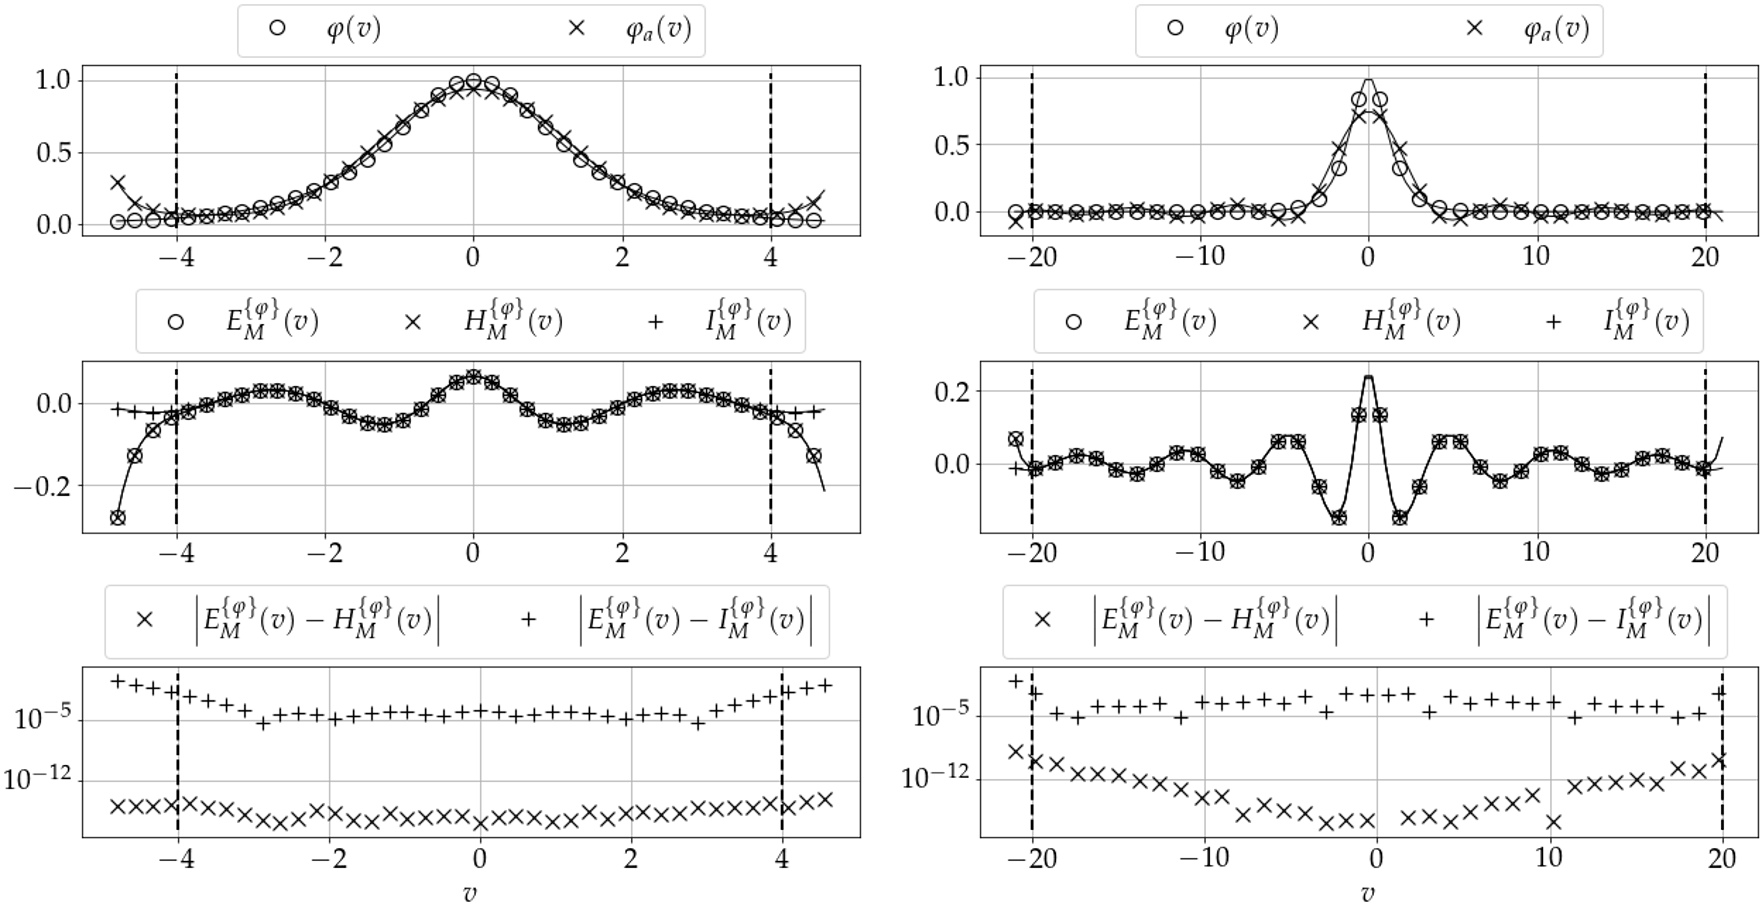
\includegraphics[width=0.95\textwidth]{Images/sech_comparison.png}
	\caption[Expansion Results and Errors for $\varphi(v) = \sech(v)$]
	{Expansion results and errors for $\varphi(v) = \sech(v)$.
		Left: number of terms  $M=8$ and validity parameter $V=4$.
		Right: number of terms  $M=25$ and validity parameter $V=20$.
		Top: expansion $\varphi_a(v)$ and true function $\varphi(v)$;
		middle: measured error $E_M^{\{\varphi\}}(v)$, exact error
		$H_M^{\{\varphi\}}(v)$, approximate error $I_M^{\{\varphi\}}(v)$;
		bottom: difference between measured errors and predicted errors.
	}
	\label{fig_sech_comparison}
\end{figure}
\begin{figure}[pb!]
	\centering
	\textit{
		Hyperbolic Tangent Expansion
	}\par\medskip
	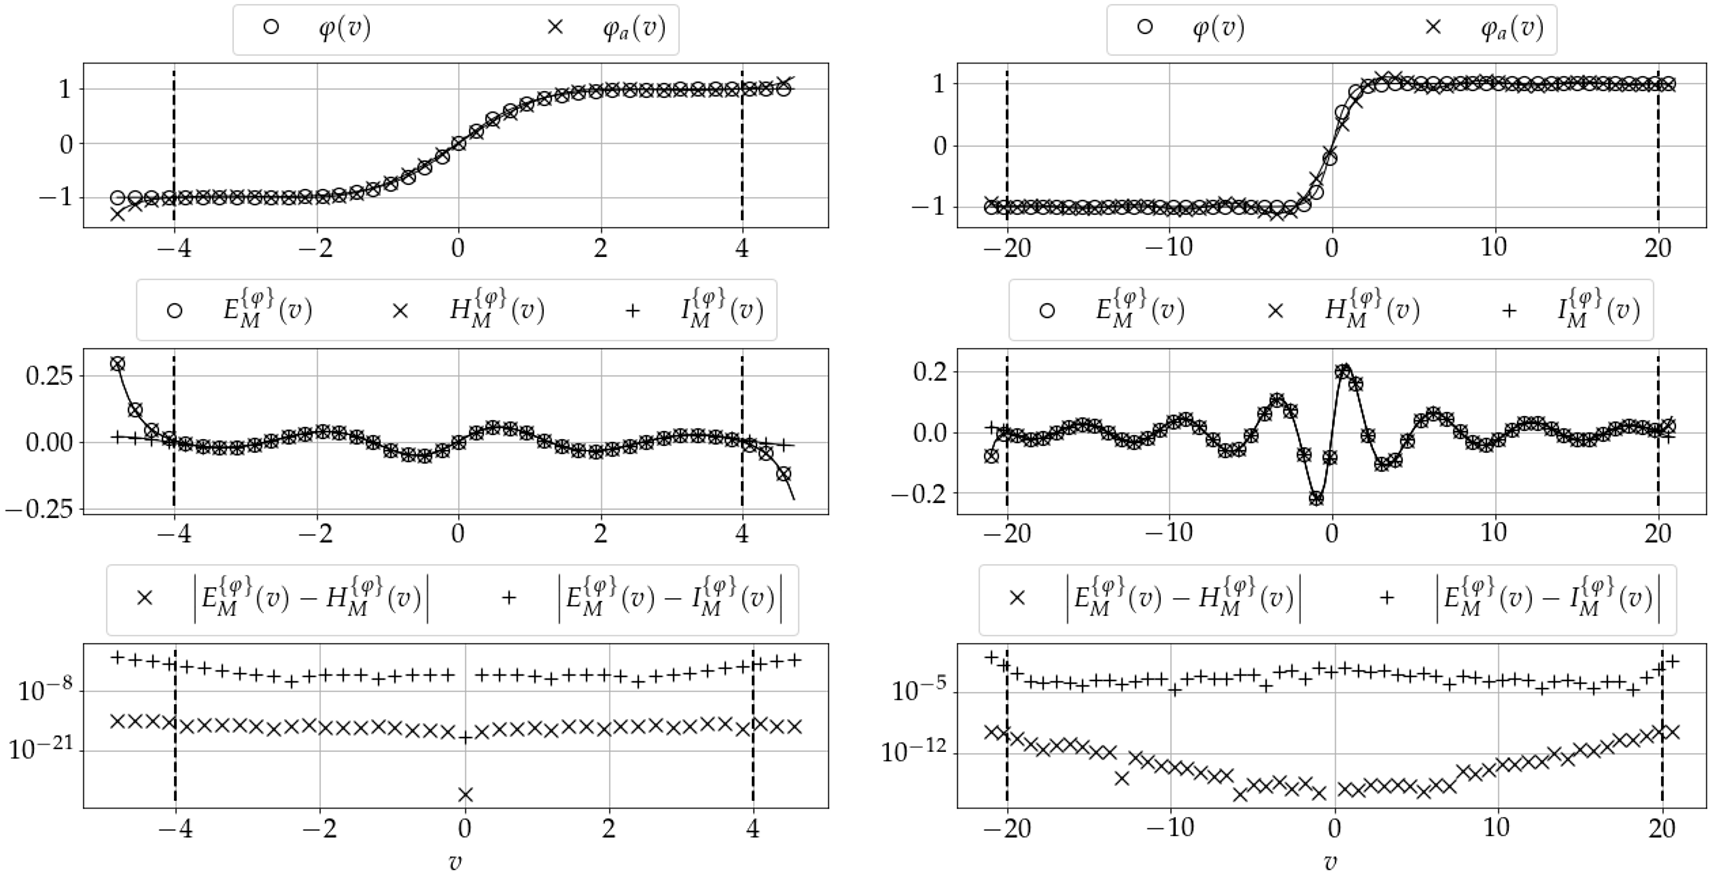
\includegraphics[width=0.95\textwidth]{Images/tanh_comparison.png}
	\caption[Expansion Results and Errors for $\varphi(v) = \tanh(v)$]
	{Expansion results and errors for $\varphi(v) = \tanh(v)$.
		Left: number of terms  $M=8$ and validity parameter $V=4$.
		Right: number of terms  $M=25$ and validity parameter $V=20$.
		Top: expansion $\varphi_a(v)$ and true function $\varphi(v)$;
		middle: measured error $E_M^{\{\varphi\}}(v)$, exact error
		$H_M^{\{\varphi\}}(v)$, approximate error $I_M^{\{\varphi\}}(v)$;
		bottom: difference between measured errors and predicted errors.
	}
	\label{fig_tanh_comparison}
\end{figure}

\begin{figure}[pt!]
	\centering
	\textit{
		Hyperbolic Secant Squared Expansion
	}\par\medskip
	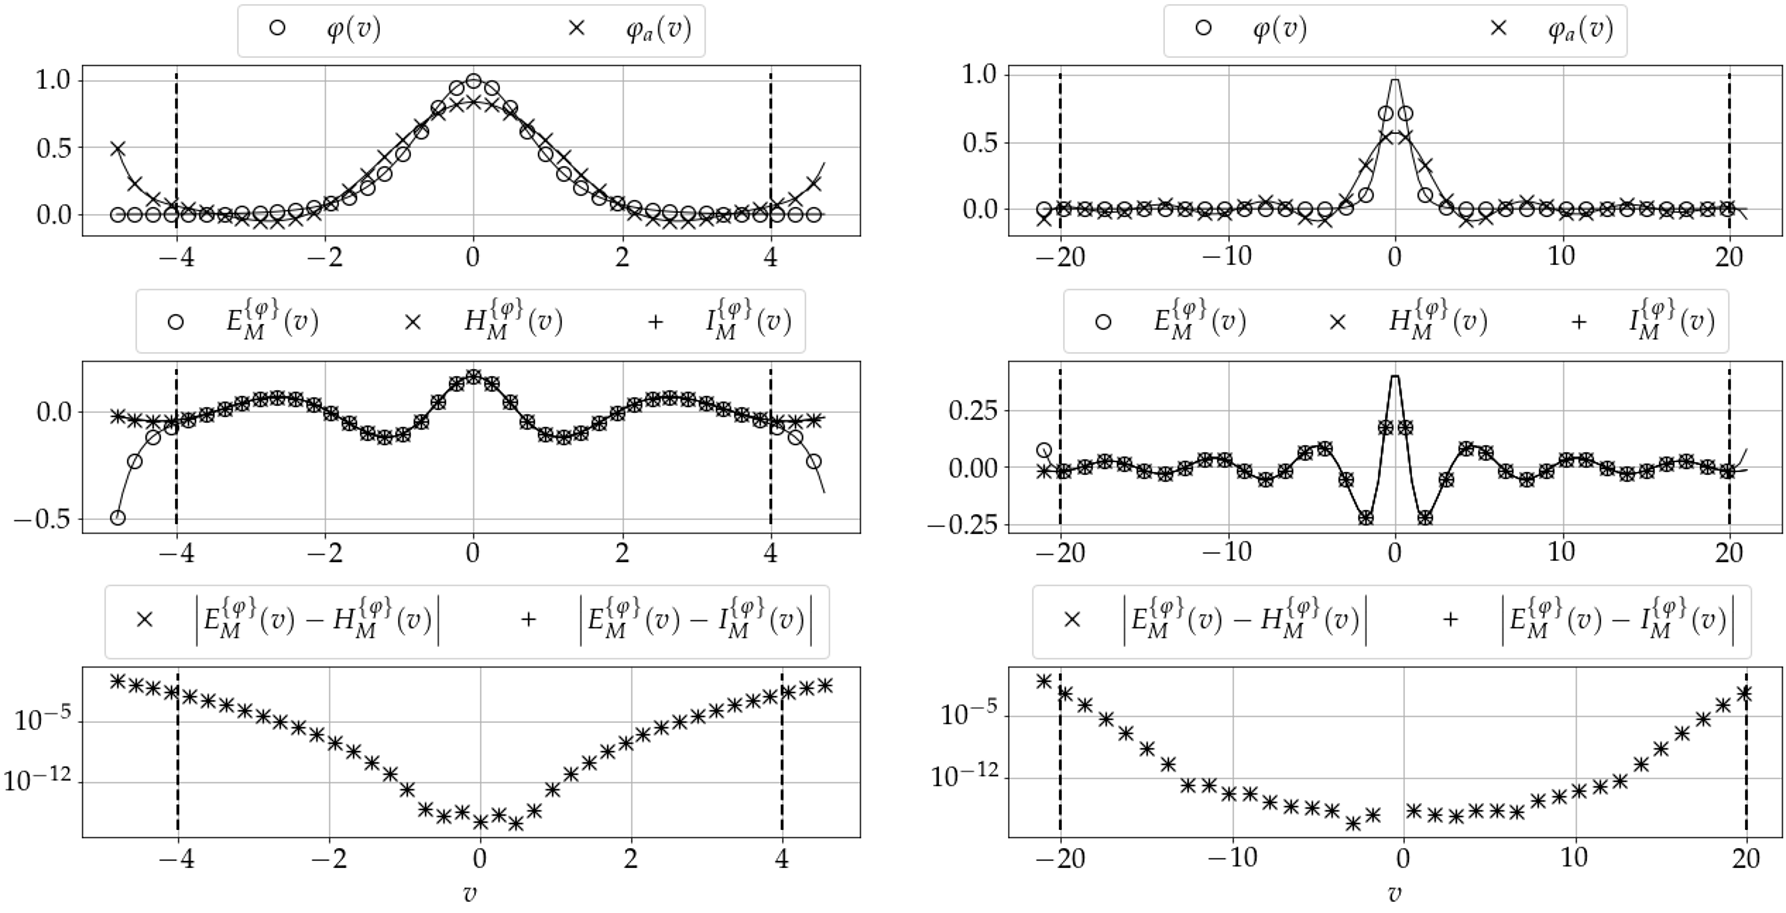
\includegraphics[width=0.95\textwidth]{Images/sech2_comparison.png}
	\caption[Expansion Results and Errors for $\varphi(v) = \sech^2(v)$]
	{Expansion results and errors for $\varphi(v) = \sech^2(v)$.
		Left: number of terms  $M=8$ and validity parameter $V=4$.
		Right: number of terms  $M=25$ and validity parameter $V=20$.
		Top: expansion $\varphi_a(v)$ and true function $\varphi(v)$;
		middle: measured error $E_M^{\{\varphi\}}(v)$, exact error
		$H_M^{\{\varphi\}}(v)$, approximate error $I_M^{\{\varphi\}}(v)$;
		bottom: difference between measured errors and predicted errors.  Note
		that $I_M^{\{\varphi\}}(v) = E_M^{\{\varphi\}}(v)$ inside $(-V, V)$ in this case
		because we only provide an exact expression for the inner error component and
		do not derive a simplified approximation.
	}
	\label{fig_sech2_comparison}
\end{figure}
\begin{figure}[pb!]
	\centering
	\textit{
		Rectified Linear Unit Expansion
	}\par\medskip
	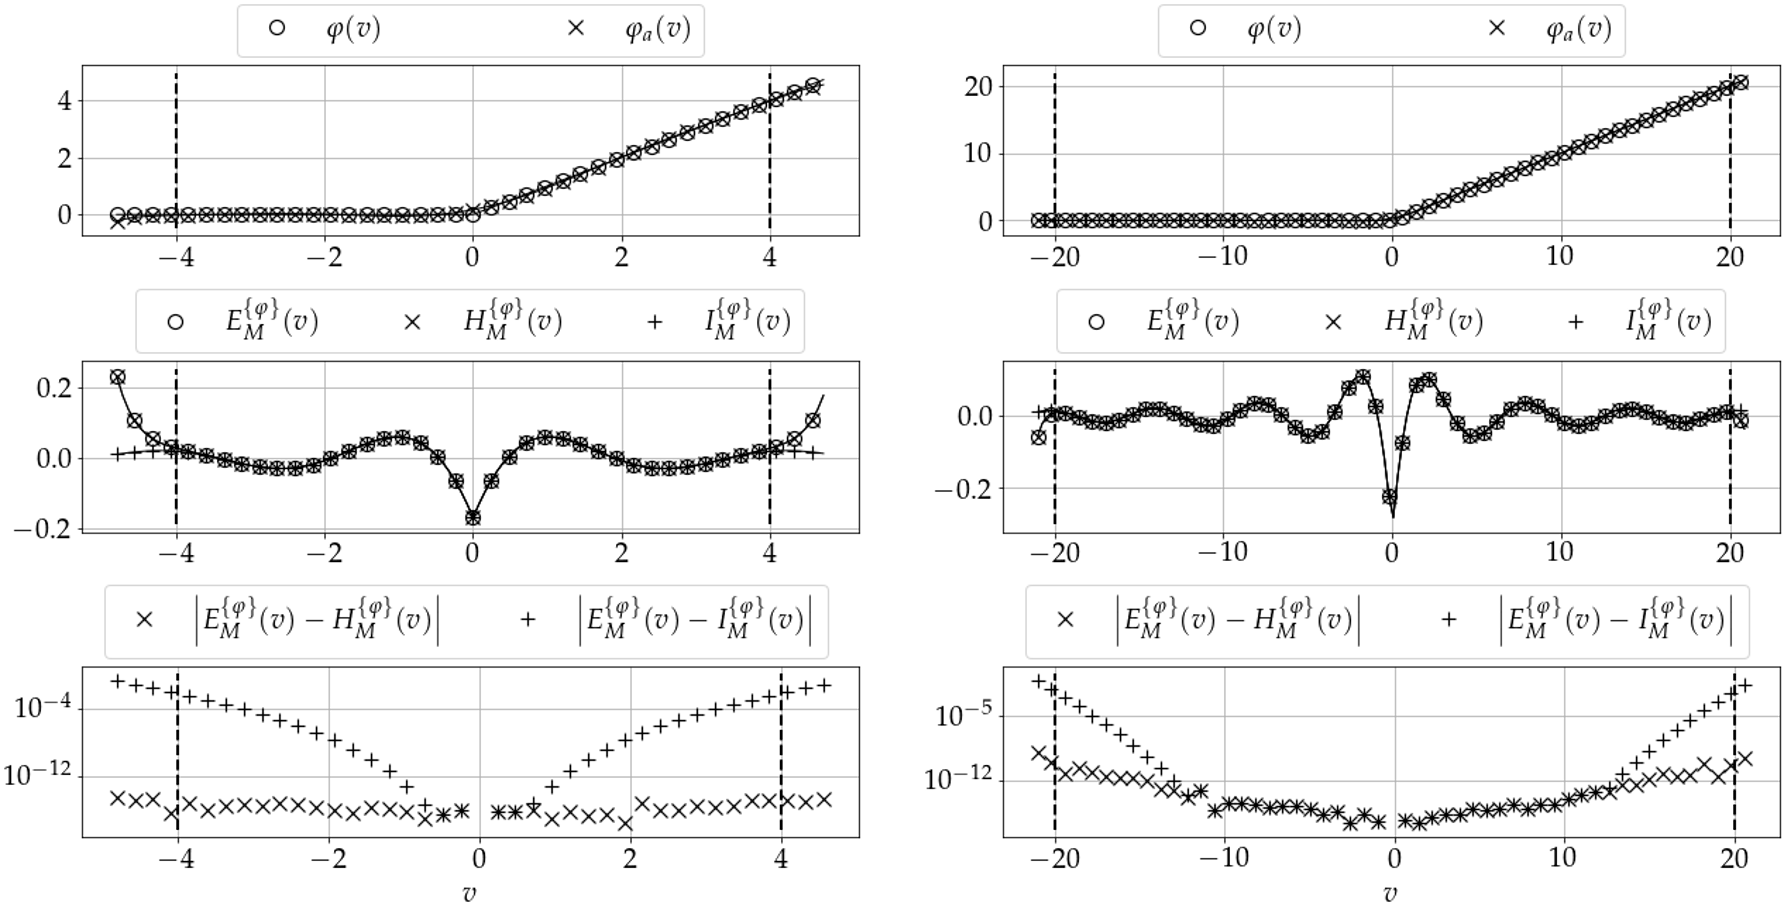
\includegraphics[width=0.95\textwidth]{Images/relu_comparison.png}
	\caption[Expansion Results and Errors for $\varphi(v) = \relu(v)$]
	{Expansion results and errors for $\varphi(v) = \relu(v)$.
		Left: number of terms  $M=8$ and validity parameter $V=4$.
		Right: number of terms  $M=25$ and validity parameter $V=20$.
		Top: expansion $\varphi_a(v)$ and true function $\varphi(v)$;
		middle: measured error $E_M^{\{\varphi\}}(v)$, exact error
		$H_M^{\{\varphi\}}(v)$, approximate error $I_M^{\{\varphi\}}(v)$;
		bottom: difference between measured errors and predicted errors.
	}
	\label{fig_relu_comparison}
\end{figure}

\begin{figure}[pbt!]
	\centering
	\textit{
		Hyperbolic Tangent Convergence Surfaces
	}\par\medskip
	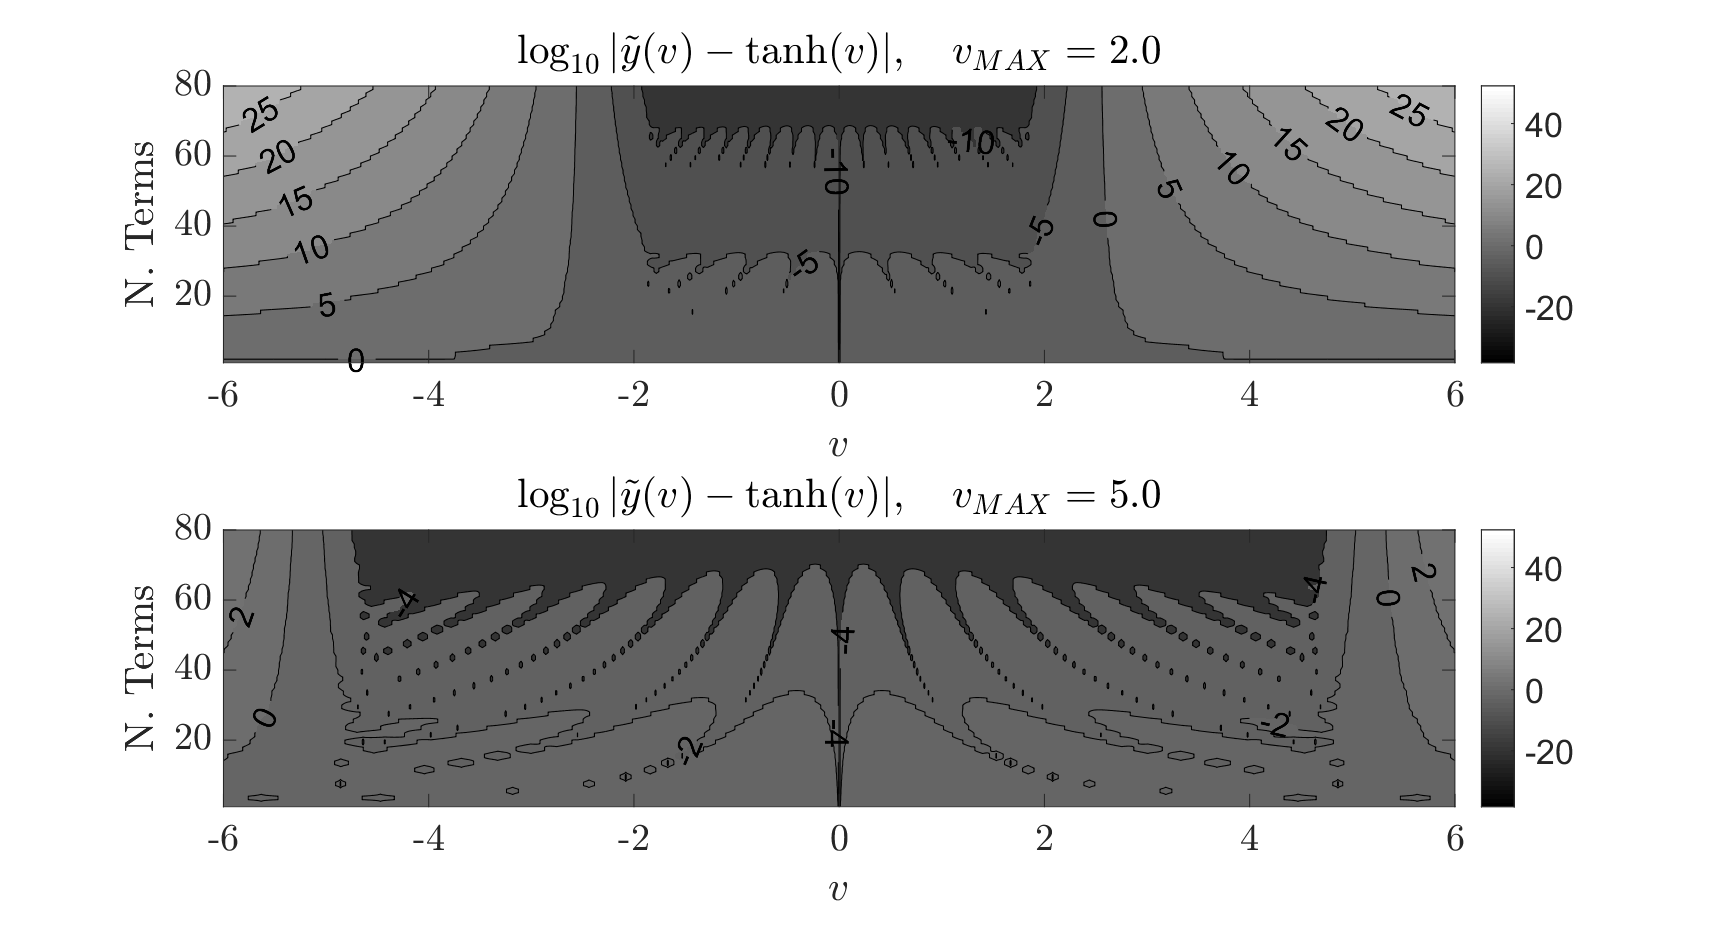
\includegraphics[width=\textwidth]{Images/ConvergenceSurfacesTanh.png}
	\caption[Convergence Surface for $\tanh(v)$]{The error between the modified expansion of the hyperbolic tangent and the true hyperbolic tangent is shown with respect to the argument $v$ and the number of terms used in the expansion.  Even powered terms which are always zero in the expansion of the hyperbolic tangent are counted in the number of terms, so 80 terms equates to $M=40$.  The expansion with $v_{MAX}=5$ has a wider region of convergence but requires more terms to reach an error as small as the expansion having $v_{MAX}=2$.  Both expansions diverge rapidly outside their regions of convergence.}
	\label{fig_tanh_convergence}
\end{figure}
